% !TeX program = lualatex
% !TeX root = main.tex
\renewcommand*{\dictumwidth}{0.5\textwidth}
\setchapterpreamble[u]{%
	\dictum[David H. Baley%\footnotemark
]{``12.  If all else fails, show pretty pictures and animated videos, and don't talk about performance.''}}

\chapter{Evaluation}
\label{chap:evaluation}
\bigskip
\textit{The final chapter deals with the evaluation of the processor model described in the second chapter,  as well as the evaluation of the extension to ResourcesUtilizationTracingLibrary from the previous chapter.}
%\footnotetext{\url{http://crd.lbl.gov/\,dhbailey/dhbpapers/twelve-ways.pdf}}

\bigskip
\lettrine[lines=2, lhang=.1, lraise=.1]{M}{easurements} of the different frequency\,/\,voltage-pairs (P-states) and their corresponding power consumption of the processor (without the other system) are hard to find, because special equipment is needed respectively the mainboard has to be modified\cite{ht4uCPU}. Even measurements with the complete system are mostly not qualified for serious comparisons. Either there are too few measurements or the test procedure is not really described.

One exception are so called ``over-clocking"-sites trying to seize the last bit of performance of a processor by using either big tower cooler, water cooling or even liquid nitrogen. This is done by rising the frequency and voltage of the processor until no stable operating is possible expressing in processor miscalculations, memory failures or complete system crashes.

\section{Processor Model Validation}
\label{sec:pmv}
To check the accuracy of the processor power consumption model, real world measurements were taken from \cite{xbit}. These measurements are from a variety of different systems with different frequency\,/\,voltage-pairs---no P-states because frequency and voltage were increased ``by hand''---for the whole system.

Because the essential power consumption equation (\ref{eq:V2f}, $P = U^2 \cdot f \cdot \alpha \cdot C$) only deals with the processor, not the complete system, the validation is based on the differences between the measured data-points and the calculated data-points to a baseline. This baseline is always the highest reached frequency, and therefore the highest power consumption of a test series.

The power consumption for the whole system consists obviously of the processor consumption and the consumption of the remaining system.
%
\begin{align*}
W &= P + S
\end{align*}
%
$W$ stands for the power consumption of the whole system, $P$ for the processor and $S$ for the system without processor. The test systems were stressed with the LINPACK frontend LinX producing load mainly on the processor (on all available cores) and some RAM. By assuming that the rest of the system is idle, or at least always utilized the same amount, it is possible to remove $S$ by writing

%
\begin{align*}
W_1 - W_2 &= (P_1 + S) - (P_2 + S)\\
			&= P_1 - P_2\\
			&=U_1^2 \cdot f_1 \cdot \alpha \cdot C - U_2^2 \cdot f_2 \cdot \alpha \cdot C\\
			&=\alpha \cdot C \cdot (U_1^2 \cdot f_1 - U_2^2 \cdot f_2)\\
\\
\Rightarrow W_1 - W_2 &= \delta \cdot (U_1^2 \cdot f_1 - U_2^2 \cdot f_2)
\end{align*}
%
All these values are available, except $\delta$. A little rearrangement of the equation above and building the mean value results in \delta:

%
\begin{align*}
\bar{\delta}  &= \frac{W_i - W_j}{U_i^2 \cdot f_i - U_j^2 \cdot f_j}
\end{align*}
%
Based upon these equation table\,\ref{tbl:ppcverification} shows the complete results of this examination. A mean variance of 4.30\,\% (6.55\,W) and maximum variance of 10.27\,\% (15.49\,W) is quite good, considering the measurements are based on whole systems and quite different processor types (dual-\,/\,quad-core, with and without uncore). The calculated results were mostly above the measured data indicating the rising temperature at those high frequencies as an additional influence. 

As already discussed in section\,\ref{sec:summary} the approximations are just as good as the amount of data they work with. Table\,\ref{tbl:approximations} based on the P-states of three real world processors shows an average difference of 0.039\,V (3.56\,\%) respectively 0.024\,V (2.10\,\%) for the gradient and intercept approaches, whereas the frequency³ approach is off by 0.28\,V (23.38\,\%). The reasons for this were discussed in section\,\ref{sec:approx} and lead to the other two approximations. Figure\,\ref{fig:modelcompare} depicts this fact.

%\todo{approximations auf summary verweisen, wiederholen, tabelle am ende}

%
%
\newpage
\section{P- and C-state Tracing Evaluation}
To examine the functionality of the implemented processor state tracing, a script generating a specific load pattern was used on a dual-core notebook enabling a visual check. The script can be found in the appendix \ref{sec:stress}. The notebook has three P-states (frequencies: 1000\,MHz, 1333\,MHz, 1833\,MHz), four C-states and runs the ondemand governor.

The load pattern consists of

%
\begin{multicols}{2}
\begin{description}
\item[00\,s] sleep for 10 seconds
\item[10\,s] CPU-load on core 1 for 20 seconds
\item[20\,s] CPU-load on core 2 for 20 seconds
\item[30\,s] stop stressing core 1
\item[40\,s] stop stressing core 2\\sleep for 10 seconds
\item[50\,s] writing 1024 MB to harddisk
\item[90\,s] terminating trace and script
\end{description}
\end{multicols}
%

\noindent
Figure \ref{fig:tracing} shows the visualization with Sunshot for the resulting trace. It shows well the changes of the P-states under load and the usage of the deep C-states in idle. While idle the trace reports nearly always the use of the C3-state, and never the C1- or even C2-state.

Writing to the harddisk shows an interesting picture. Usage of C3 is still very high, with some activity in C0 and idling in C2 (C1 is again unused), though the utilization of core 1 shows always 100\% and core 2 has phases of high utilization, too. 
P-state usage for core 1 is rather high, whereas core 2 is approximately half the time in the lowest P-state.

After finishing writing, the last 10 seconds show again some idle time with nearly 100\,\% C3- and lowest P-state-usage.

%Average utilization matches average frequency nearly perfect: 
%\begin{align*}
%0\,\% &\equiv 1000 \text{MHz}&100\,\% &\equiv 1833\,\text{MHz}\\
%\Rightarrow 66.67\,\% &\equiv 1555 \text{MHz}&46.40\,\% &\equiv 1387\,\text{MHz}
%\end{align*}

%\subsection*{Utilization vs. C0-usage}

\superpar
As seen in figure\,\ref{fig:tracing} utilization of one core matches always C0-usage, except while writing to harddisk. But utilization is actually the C0-usage, so they should be exactly the same.

The utilization $u_{CPU}$ in the time interval $[t_{i-1}, t_i]$ is calculated with

%
\begin{align*}
u_{CPU}(t_{i-1}, t_i) =& 1-\frac{x_{idle}(t_i) - x_{idle}(t_{i-1})}{x_{total}(t_i) - x_{total}(t_{i-1})}
\end{align*}
%
whereas $x_{idle}(t_i)$ is the time spent in idle and $x_{total}(t_i)$ the total elapsed time since system start\cite{krempel}. There is no difference in the formula which was used in section\,\ref{sec:rutl}:
%
\begin{align*}
percentage\,Cn &=  \frac{\text{time in } Cn}{\text{\lstinline!interval_length!}} \cdot 100
\end{align*}
%
$x_{idle}(t_i)$ and $x_{total}(t_i)$ are provided by libgtop\cite{libgtop}, which presents the values of \lstinline!\proc\stat!, which delivers statistics of the kernel and the system. Statistics for the CPU are the times spent in different situations since system start:

%
\begin{multicols}{2}
\begin{description}
\item[user] normal processes executing
\item[nice] niced processes executing
\item[system] processes in kernel mode
\item[idle] twiddling thumbs
\item[iowait] waiting for I/O to complete
\item[irq] servicing interrupts
\item[softirq] servicing softirqs
\end{description}
\end{multicols}
%

\noindent
While watching the tracing progress with \lstinline!vmstat!, which also uses \lstinline!\proc\stat!, idle counter stalls and \lstinline!iowait! increases, as expected. After checking the code segment of libgtop which is in charge of providing the values from \lstinline!\proc\stat!, the different results in tracing the utilization and the C0-usage are becoming clear. Libgtop reads from \lstinline!\proc\stat! and sums the values up to provide $x_{total}(t_i)$.

In order to get the full idle time, the above equation has to use $x_{iowait}(t_i)$ too.

%
\begin{align*}
u_{CPU}(t_{i-1}, t_i) =& 1-\frac%
{x_{idle}(t_i) + x_{iowait}(t_i) - x_{idle}(t_{i-1}) - x_{iowait}(t_{i-1})}%
{x_{total}(t_i) - x_{total}(t_{i-1})}
\end{align*}
%
Figure\,\ref{fig:bugfree} shows the visualization of the same load pattern with the adjusted version of the tracing library. Utilization now equals C0-usage.

% 
\begin{table}[hb]
	\caption[Tracing Statistics on notebook]{Tracing Statistics on notebook---average values across the whole trace}
	\label{tbl:statistics}
	\centering
	\begin{tabular}{*{7}{c}}
\hiderowcolors
		\toprule			
			&C0\,[\%]&C1\,[\%]&C2\,[\%]&C3\,[\%]&frequency\,[MHz]&utilization\,[\%]\\
		\midrule
\showrowcolors
			core 1&27.50&0.00&5.84&66.12&1392&26.11\\
			core 2&26.41&0.03&6.42&66.37&1375&25.66\\
		\bottomrule
	\end{tabular}
\end{table}
%



\noindent
Table \ref{tbl:statistics} shows that the coverage of the C-states is 99.46\,\% respectively 99.23\,\%. The missing 1 percent is the failure given the slightly varying interval times and of course some rounding mistakes. The difference between utilization and C0-usage is now very low, but still there. This will be rechecked after using the exact interval times.

%
\begin{sidewaysfigure}[h]
	\centering
	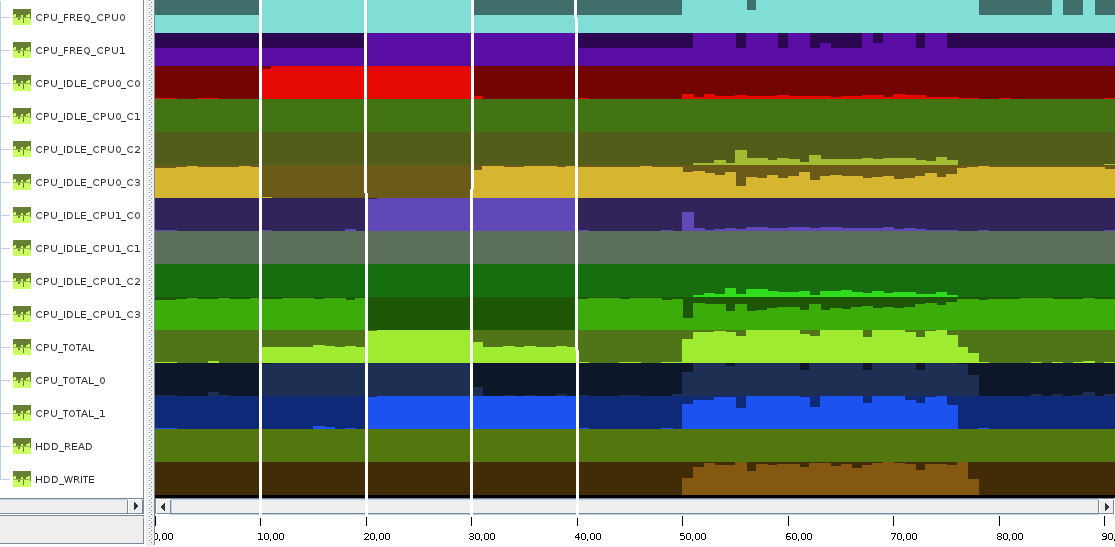
\includegraphics[width=\linewidth, height=\textheight, keepaspectratio]{pix/bug}
	\caption{Tracing screenshot showing utilization bug}
	\label{fig:tracing}
\end{sidewaysfigure}
%
\begin{sidewaysfigure}[h]
	\centering
	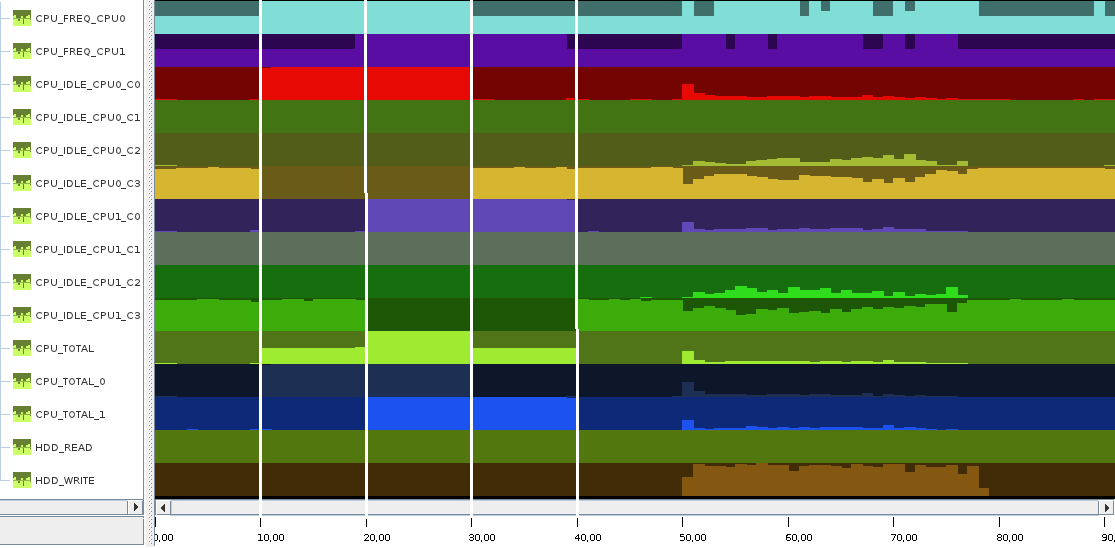
\includegraphics[width=\linewidth, height=\textheight, keepaspectratio]{pix/bugfree}
	\caption{Tracing screenshot without utilization bug}
	\label{fig:bugfree}
\end{sidewaysfigure}
%
\clearpage

%
%
%\section{Power Consumption Estimation Model}

%
%
\chapter{Conclusion and Future Work}
\enlargethispage{5\baselineskip}
Reducing power consumption is important. First step is always to measure what consumes when the most. It is usually not possible to measure every component of every node in a cluster. Because of that, a model has been presented calculating the power consumption of a processor based on its frequency and voltage. The resulting equation $P_2 = P_1 \cdot \frac{U_2^2 \cdot f_2}{U_1^2 \cdot f_1}$ needs a baseline measurement for $P_1$ at frequency $f_1$ and voltage $U_1$. The further three approximations can be used when voltage tracing is not (fully) available.
Evaluation showed this is a usable way of estimating. Taking many different overclocked systems measured with different frequency-\,/\,voltage-pairs (no P-states) resulted in a mean variance of 4.30\,\% (6.55\,W) and maximum variance of 10.27\,\% (15.49\,W) using this model. The approximations were evaluated with the P-states of three processors. The frequency³ approach, based purely on the frequency, showed a mean difference of 23.38\,\%, whereas the other two (intercept and gradient approaches) based on more information involving the characteristics of the P-states were rather good with mean differences of 3.56\,\% respectively 2.10\,\%.

In order to use this model, the appropriate values have to be recorded. To do so, an existing tracing library was extended to log the P- and C-states of a processor using the kernel subsystems CPUFreq and CPUIdle. Visual inspection and the evaluation showed reasonable results. 

A power estimator was implemented using the resulting trace files to finally gather the power respectively energy consumption of the processor based on the presented model. The estimator resembles the design of CPUFreq\,/\,CPUIdle allowing easy combination of different processor types and analysis strategies.

\superpar
Future work consists of improvements to the model by measuring the impact of the temperature change and the consumption of the uncore-part of the CPU.

ResourcesUtilizationTracingLibrary has to be further extended to include the usage of the real elapsed time for calculating the active processor time, and voltage tracing with IPMI has to be implemented.

Later improvements also include merging the power estimator into HDPowerEstimation and considering the amount of state-changes for a more detailed power consumption, as well as developing strategies to predict energy saving potential on hardware not using energy saving mechanisms.\\[1em]
All together, it shows that this approach is a reasonable and working way to estimate the power consumption used by the processor.